\section{Installazione}
Per installare il prodotto\glosp è necessario scaricare il contenuto di questi moduli del repository:
\begin{itemize}
	\item 
\end{itemize}
Terminato lo scaricamento si può procedere all'installazione

\subsection{Applicazione di addestramento esterna}
Per far partire l'applicazione esterna bisogna semplicemente avviare l'eseguibile fornito. Di seguito viene illustrato come.
	\subsubsection{Windows}
	Aprire la cartella "grafana\_configuration\_utility" e fare doppio click sul file "grafana\_configuration\_utility.exe" e si aprirà l'applicazione per l'addestramento.

	\subsubsection{macOS e GNU/Linux}
	\begin{itemize}
		\item aprire la cartella "grafana\_configuration\_utility";
		\item assicurarsi che il file "grafana\_configuration\_utility.sh" sia eseguibile in uno dei modi seguenti:
		\begin{itemize}
			\item fare click con il tasto destro sul file, selezionare proprietà e poi permessi e mettere la spunta su "eseguibile";
			\item aprire un terminale nella cartella "grafana\_configuration\_utility" e dare il seguente comando: 
			\begin{verbatim}
			chmod +x grafana\_configuration\_utility.sh
			\end{verbatim}
		\end{itemize}
		\item aprire un terminale nella cartella BLABLABLA e dare il seguente comando:
		\begin{verbatim}
	    .\grafana_configuration_utility.sh
		\end{verbatim}
	\end{itemize}
\subsection{Grafana}
Per installare Grafana\glo, visitare la pagina \url{https://grafana.com/get}. Qui è possibile trovare il download per macOS, Windows e sistemi operativi GNU/Linux.
\subsubsection{Eseguire il servizio WEB Grafana} Per eseguire il servizio WEB Grafana\glo, aprire la cartella "bin" dell'installazione Grafana\glosp ed a seconda del sistema operativo eseguire:
\begin{itemize}
	\item \textbf{Windows}: doppio click sul file "grafana-server";
	\item \textbf{Linux e Mac}: eseguire in una shell il comando:
	\begin{verbatim}
	./grafana-server web
	\end{verbatim}
\end{itemize}
Collegarsi quindi con un browser all'indirizzo \url{http://localhost:3000/}. Le credenziali richieste al primo avvio sono username "admin" e password "admin".
\begin{center}
	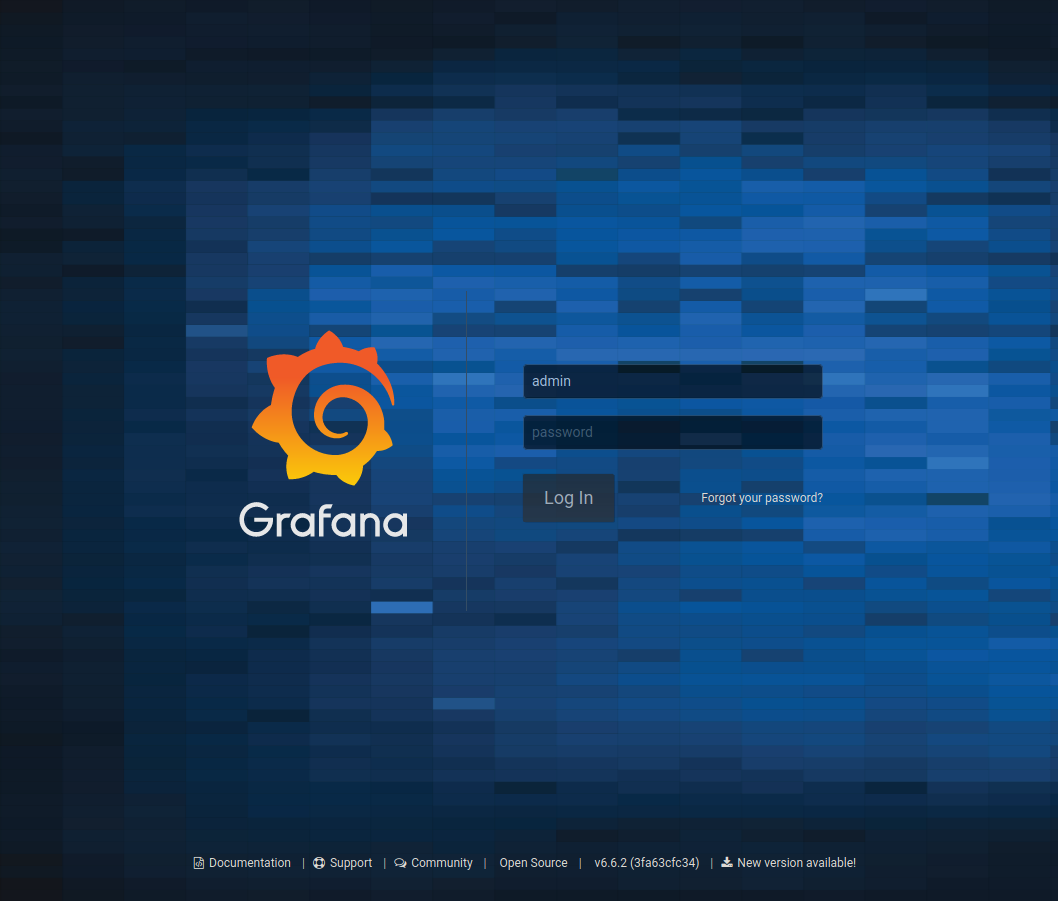
\includegraphics[width=10cm,height=\textheight,keepaspectratio]{img/grafana-login.png}
\end{center}

\subsection{Plug-in di Grafana}
Per poter utilizzare il plug-in bisogna copiare la cartella "grafana\_prediction\_plugin" (scaricata dal link a inizio sezione) all'interno della cartella "data/plugins" dell'installazione Grafana\glo. \\
Bisogna poi trovare il plug-in "Grafana prediction plugin"
\begin{center}
	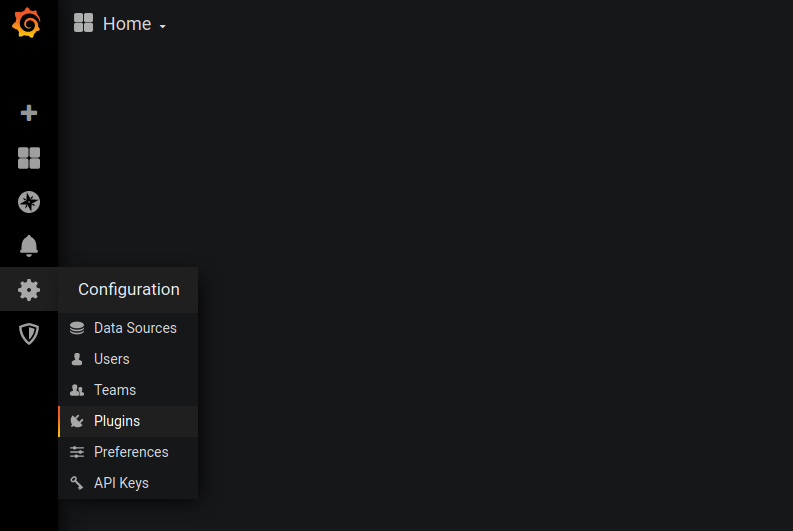
\includegraphics[width=10cm]{img/inserimento-plugin1.png}
\end{center}

\begin{center}
	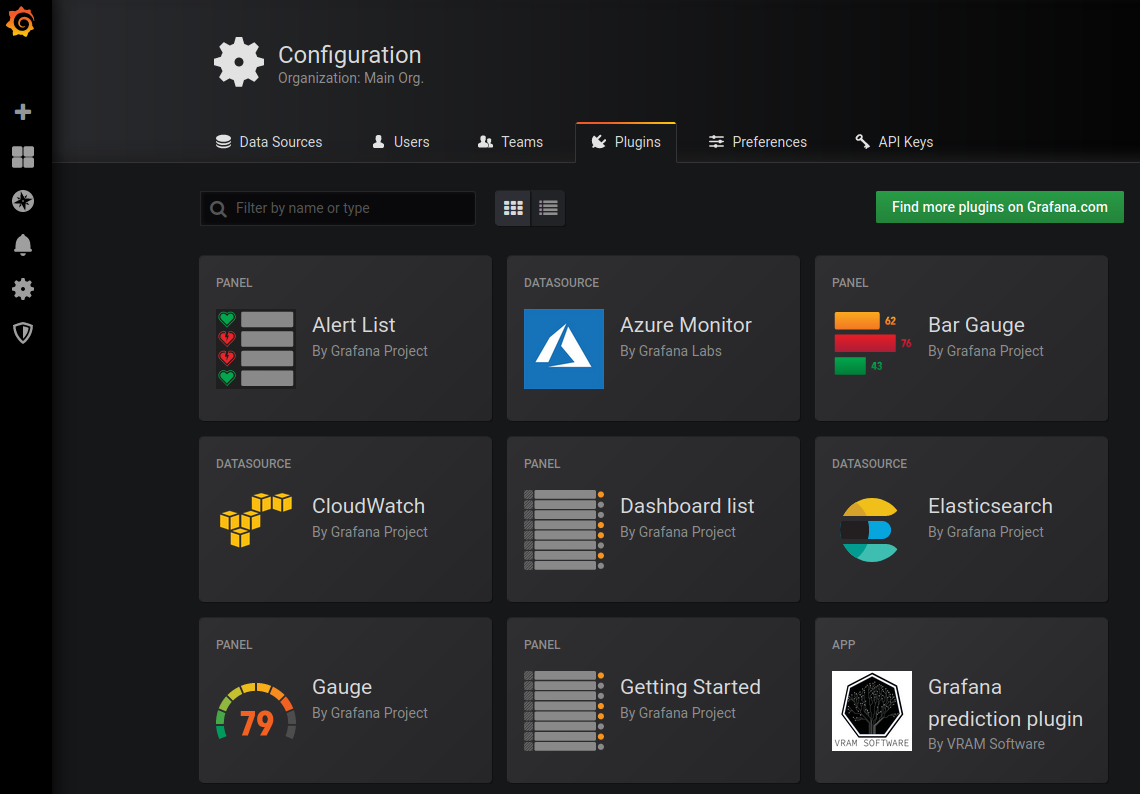
\includegraphics[width=10cm]{img/inserimento-plugin2.png}
\end{center}

Infine è necessario abilitare il plug-in: una volta cliccato su "Grafana prediction plugin", sarà sufficiente aprire la tab "Config" e cliccare sul pulsante "Enable".

\begin{center}
	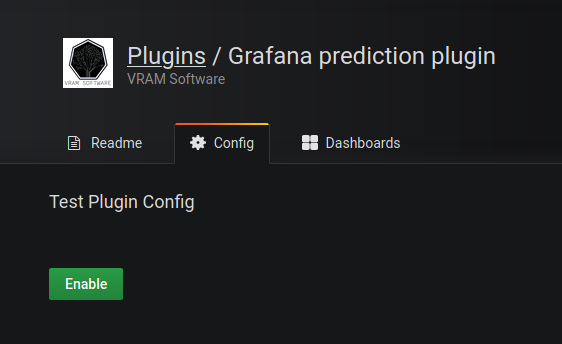
\includegraphics[width=10cm]{img/inserimento-plugin3.png}
\end{center}

